As for results, the data from heart disease rendered the figure \ref{fig:cluster_free_3s}. In this, we focused on continuous variables only. For easier reading, the data is as shown in the table \ref{tab:datapoints}. We used data from the real world to test if everything would work similarly, rendering the image \ref{fig:cluster_mydata_9s}. We added a binary category to show how meaningless the value turn in order to get any information out of it.




%TC:ignore

\begin{figure}[htpb]
\centering
\captionsetup{justification=centering}
\caption[Clustering for 3 continuous variables with 3 silos]{Clustering for 3 continuous variables with 3 silos and true centroids (S2) and true means (S2) for example purposes; The values were normalized for visualization purposes with MinMax}
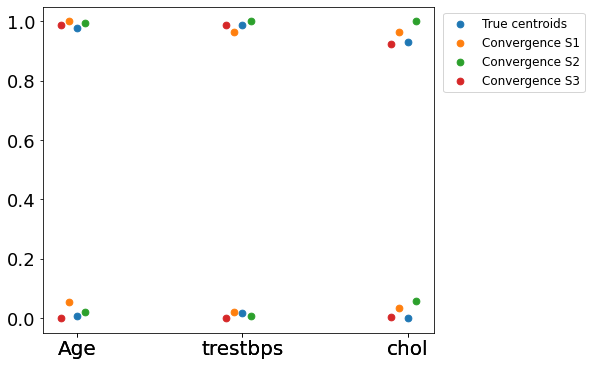
\includegraphics[scale=0.50]{figures/my_cluster_3.png}
\label{fig:cluster_free_3s} 
\end{figure}



%TC:endignore
\begin{table}[htbp]
\centering
 \setlength{\tabcolsep}{7pt} % Default value: 6pt 
 \renewcommand{\arraystretch}{1.35} % Default value: 1
  \captionsetup{justification=centering} 
\caption[Final Data points after convergence of clustering]{Final Data points after convergence; S1, S2 and S3 are the centroids obtained in each silo (S) after convergence; True centroids are the centroids of the true means of all silos (TC)}
\label{tab:datapoints}
\begin{tabular}{l|ccc}
\toprule
 & Age & trestbps & chol \\
\midrule
S1 & 46.3 , 61.1 & 121.1 , 148.9 & 218.9 , 300.8 \\
S2  & 45.8 , 61.0 & 120.7 , 149.9 & 220.9 , 304.0 \\
S3 & 45.5 , 61.0 & 120.5 , 149.6 & 216.1 , 297.4 \\
TC  & 45.6 , 60.8 & 121.0 , 149.6 & 215.8 , 297.9   \\

\bottomrule
\end{tabular}
\end{table}




%TC:ignore



\begin{figure}[H]
\centering
\captionsetup{justification=centering}
\caption[Clustering for 3 variables with 9 silos]{Clustering for 3 variables with 9 silos and true centroids of the true means (TC); 2 continuous and 1 categorical one hot encoded, The values were normalised for visualisation purposes with MinMax}\label{fig:cluster_mydata_9s} 
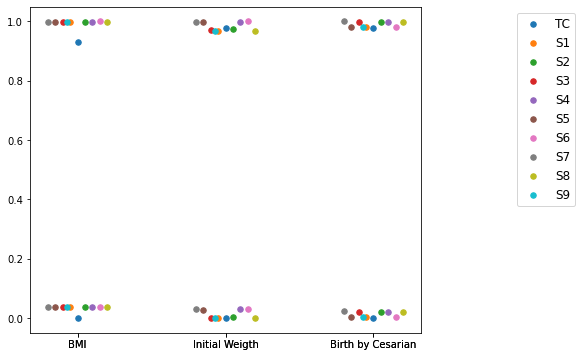
\includegraphics[scale=0.60]{figures/my_cluster_9.png}
\end{figure}
%TC:endignore

As before, the data is in table format in \ref{tab:datapoints_9}.

%%True Centroid & 24.9 , 25.3 & 66.6 , 65.6  & 0.24 , 0.29 \\

\begin{table}[htbp]
\centering
 \setlength{\tabcolsep}{7pt} % Default value: 6pt 
 \renewcommand{\arraystretch}{1.35} % Default value: 1
  \captionsetup{justification=centering} 
\caption{Final Data points after convergence and true centroids of the true means of each silo (TC)}
\label{tab:datapoints_9}
\begin{tabular}{l|ccc}
\toprule
 & BMI & Initial Weight & Birth by Cesarian \\
\midrule
TC & 24.9 , 383.1 & 60.5 , 85.0  & 0 , 1 \\
S1 & 40.1 , 409.4 & 60.4 , 85.0 & 0.96 , -0.04 \\
S2 & 40.1 , 410.4 & 61.7 , 86.3 & 0.99 , -0.01 \\
S3 & 40.0 , 410.4 & 61.9 , 86.5 & 0.96 , -0.04 \\
S4 & 40.6 , 411.3 & 61.9 , 86.5 & 0.96 , -0.04 \\
S5 & 40.0 , 410.4 & 60.5 , 85.1 & 1.0 , 0.0 \\
S6 & 40.1 , 409.3 & 60.4 , 84.9 & 1.0 , 0.0 \\
S7 & 40.7 , 411.3 & 60.5 , 85.0 & 0.96 , -0.04 \\
S8 & 40.0 , 410.4 & 86.5 , 61.9 & 1.0 , 0.0 \\
S9 & 41.0 , 410.4 & 85.0 , 60.4 & 1.0 , 0.0 \\
\bottomrule
\end{tabular}
\end{table}




Then we experimented with categorical variables. Figure \ref{fig:cluster_3_cat} shows the convergence of the silos with proportion data and K-means with that and with K-modes.
\begin{figure}[ht]
\caption{Clustering for 3 variables with 3 silos - (A) categorical variables with  proportion with K-Means and (B)  Categorical with K-modes  }\label{fig:cluster_3_cat} 
  \subcaptionbox*{(A)}[.60\linewidth]{%
    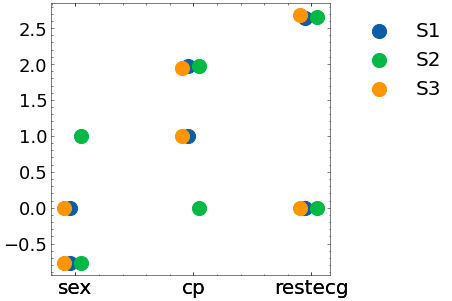
\includegraphics[width=\linewidth]{figures/my_cluster_3_cat.png}%
  }%
  \hfill
  \subcaptionbox*{(B)}[.44\linewidth]{%
    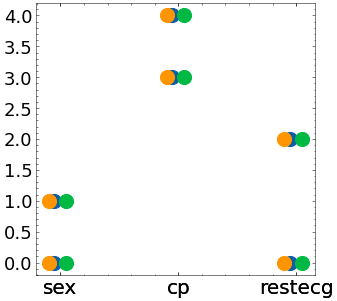
\includegraphics[width=\linewidth]{figures/my_cluster_3_cat_kmodes.png}%
  }
\end{figure}

